\documentclass{article}
% \usepackage{showframe}
\usepackage{siunitx}
\usepackage{booktabs}
\usepackage{graphicx}
\usepackage{amsmath}
\usepackage{mathtools}
% \usepackage{minted}
\usepackage{tabularx}
\usepackage{url}
% \usepackage{subfig}
% \usemintedstyle{xcode}

% \usepackage{fullpage}

\frenchspacing
% \setlength{\parindent}{0ex}
% \setlength{\parskip}{3 ex plus 2 ex minus 1 ex}

\title{Homework 10}
\author{Josh Bradt}
\date{April 28, 2016}

\begin{document}

\maketitle

Rather than running the provided code, I chose to write my own version of it. I ran this code using a matrix of dimension \num{16384} by \num{16384} with striping factors of 0, 16, and 32, as instructed. I ran on Blue Waters, compiled my code with the default Cray compiler, and requested 64 nodes to run on, for a total of 1024 processes (16 per node). The three cases were run as separate jobs, so it is likely that they ran on different sections of the machine.

\begin{figure}
    \centering
    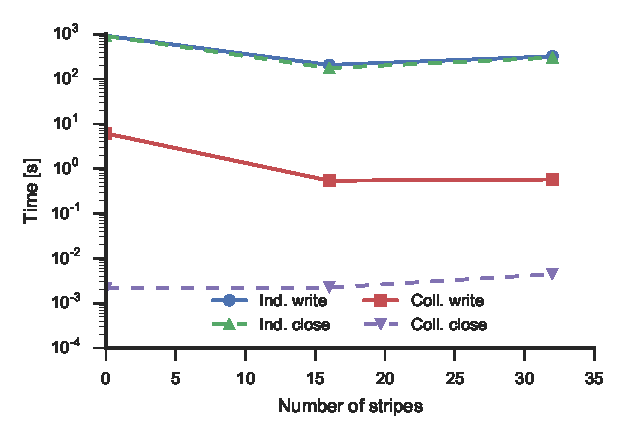
\includegraphics{times.pdf}
    \caption{The time taken for each set of parameters. Both the time to write to the file and the time to close the file are shown.}
    \label{fig:times}
\end{figure}

\begin{table}
    \centering
    \begin{tabular}{S[table-format=2]
                    c
                    S[table-format=1.4e+2]
                    S[table-format=1.4e+2]
                    S[table-format=1.4e+2]}
        \toprule
        {Num. Stripes}  & {Method}    & {Write Time [s]} & {Close Time [s]} & {Rate [B/s]} \\ \midrule
        0               & Collective  & 6.123e+00        & 2.172e-03        & 3.507e+08    \\
        0               & Independent & 9.209e+02        & 9.070e+02        & 2.332e+06    \\
        16              & Collective  & 5.403e-01        & 2.227e-03        & 3.975e+09    \\
        16              & Independent & 2.057e+02        & 1.755e+02        & 1.044e+07    \\
        32              & Collective  & 5.747e-01        & 4.449e-03        & 3.737e+09    \\
        32              & Independent & 3.194e+02        & 3.009e+02        & 6.723e+06    \\
        \bottomrule
    \end{tabular}
    \caption{Output of the code for the given parameters.}
    \label{tab:results}
\end{table}

The results of running the code are shown in Figure~\ref{fig:times} and Table~\ref{tab:results}. For all cases, the write times for the collective method were 2 to 3 orders of magnitude faster than the independent method. The close times were 5 orders of magnitude faster for the collective method than the independent method, though that result is slightly suspect since I was getting some I/O errors during the calls to the independent methods. (That being said, they still appeared to write the output to disk, so I'm not sure what was going on.)

Striping the files improved the write speeds by between 0.5 and 1 order of magnitude, so this is clearly an important optimization to make in an I/O-heavy application. Striping did, however, increase the amount of time taken to close the file after the collective write operation, but this increase is trivial when compared to the amount of time spent writing to the file, so it doesn't seem like a big problem.

\end{document}
